\section{An Illustrative Example} 
\label{sec:example}

We define a simple authomous underwater vehicle (AUV) mission that 
will illustrate potential issues arising with dynamic goal emergence
and motivate our apprach. In this domain we have an AUV that can do
two specific actions: Go from one location to another within the
water mass and survey a location in order to sample data of a feature of
interrest such as a vent similar to the one depicted in
Fig. \ref{fig:ex:axial}. Our domain is illustrated in
Fig. \ref{fig:ex:graph}, the vheicle is deployed initially with the
science objective to sample the {\em Vent 2} and the operational goal
to be back at the {\em Surface} by the end of the mission which lasts
12 hours. 

\begin{figure}[!htb]
  \centering
  \subfloat[\small Bathymetry of vent sites off of NW United States]{\label{fig:ex:axial}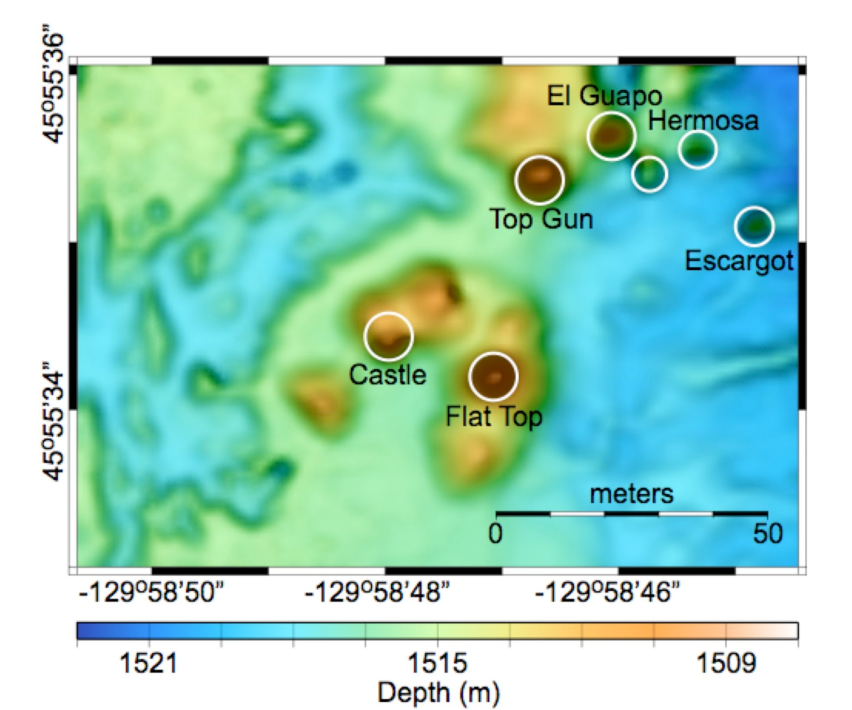
\includegraphics[scale=0.35]{figs/vents.pdf}}\\
  \subfloat[\small An illustration of our domain]{\label{fig:ex:graph}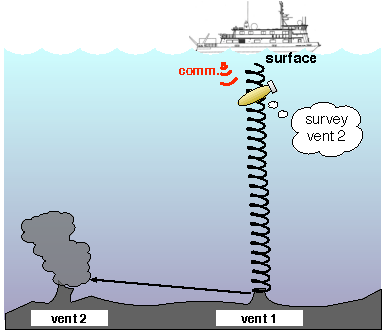
\includegraphics[width=0.51\columnwidth]{figs/auv_example}}
  \hfill \subfloat[\small Initial  problem]{\label{fig:ex:init}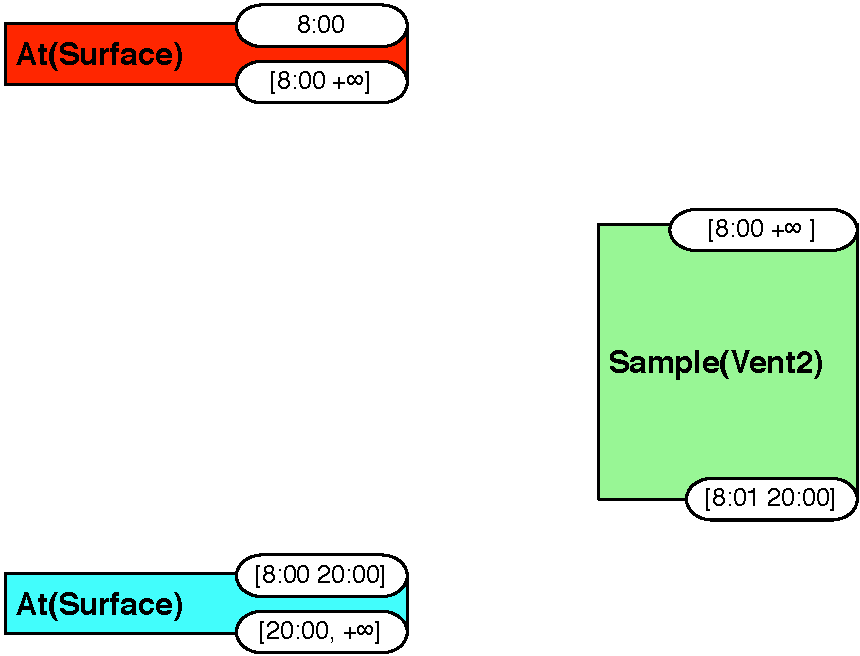
\includegraphics[width=0.47\columnwidth]{figs/example_initial}}
  \caption{\small{\ref{fig:ex:axial} shows bathymetry of actual vent
      sites off the coast of Oregon. (\ref{fig:ex:graph}) illustrate 
      the domain along with the initial partial plan for
      this problem (\ref{fig:ex:init}). In this domain our AUV is
      initially at {\em Surface} at 8am snd the mission will complete
      by 8pm.}}
\label{fig:Example}
\end{figure}

Given this initial problem (Fig. \ref{fig:ex:init}) the AUV planner
produces the flexible plan given in Fig. \ref{fig:ex:plan} which can
then be executed by the system. However, at any time during the
mission scientists can decide for example that they also want to {\em
  sample} {\em Vent 1} (for exmaple due to the processing of the data
the AUV sent through the accoustic link while flying above this
location). Such possibility raises the issue of balancing the
decisions during plan execution between staring one plan action as
early as possible --- which we will call {\em proactive} -- or wait
until the action should necessarily start -- called later. There is a 
clear difference between the two approaches but when should, for 
example, the AUV wait or start early and how either will impact the
mission execution when the new objective will be integrated by the 
AUV ? 

\begin{figure}[!htb]
  \centering
  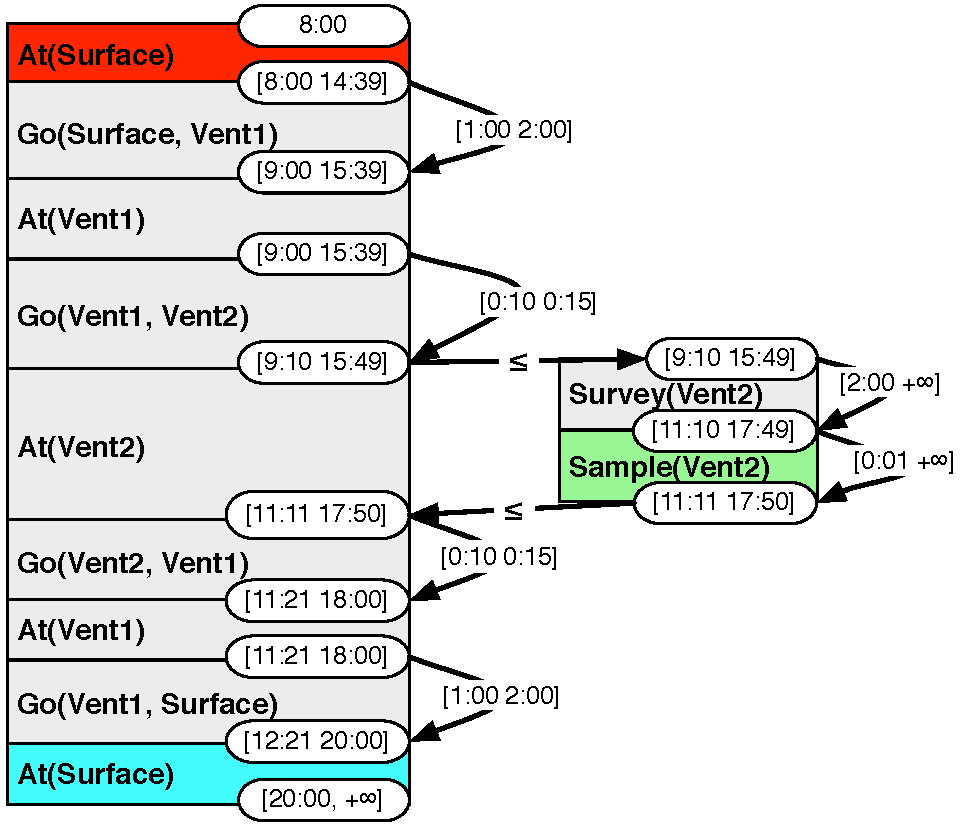
\includegraphics[width=0.8\columnwidth]{figs/example_plan}
  \caption{\small The flexible plan solution of the AUV domain in
    Fig. \ref{fig:Example}}
  \label{fig:ex:plan}
\end{figure}

{\em Deferring} all the actions is obviously not acceptable as 
it results the vehicle sitting at the surface for the most part of the
mission and starting to diving only at the very last minute (14:39 in
our plan). As a result if the new goal arrives after this time there's
no time left to do both objectives and the probot will have to exclude
one of the two science goals or fail to be at the surface by
20:00. While better, the {\em proactive} approach is still not
optimal. Indedd in that case the vehicle will skim through al the
action of the plan and be back at the surface by 12:21. If we still
consider that scientists still provide this new goal by 14:00  it
means that vehicle  will then have to dive back underwater in order to
survey and sample {\em Vent 1}. Eben though the plan didf initial
provide a solution optimal in term of makespan the resulting mission
scenario is not anymore as the vehicle went back and forth during the
mission. Moreover in this specific case the Vents are $1500 m$ deep
which result on 2 actions of at least 1 hour each that could have been
avoided should the new goal have been received while the AUV was still 
near the ocean floor. 

None of these 2 approaches are satisfactory; {\em defer} actions
result on the plan execution not being robust to the addition of new
goals while blind {\em proactive} execution can result on redundant
actions within the mission that negatively impact the ability of the
robot to do as much as it could. A more balanced execution policy
would have been for the executive to alter betwen the two policies
during the mission. 

Looking back at our initial objective we can note that these are
different by their source and nature; while 
sampling {\em vent 1} was reflecting a scientist need which served the
puropose of the mission, the goal to be back at the surface was more
related to the operators requirements in order to have regular
operation hours and not risk to lose the vehicle before its battery
ran out. While fullfilling these two goals is equallly important for
the mission success they do not have the same notion of urgency. While
it is desirable  for the AUV to go sample the {\em vent} as early as
possible, there is no strong motivation to hurry and go back to the
surface before we are gettong close to the end of the day. Therefore a
better policy for the executive is to alternativelly switch between
the two policies depending on what objective(s) they contribute to. By
doing so the resulting mission would have been for the vehicle to be
{\em proactive} until it starts to {\em Survey} the {\em Vent 2} and
then {\em defer} to go back at the surface -- meanning that it would
continue to {\em Survey} the same place -- until it either receive the
new goal to sample {\em Vent 2} or it is really time to go back to the
{\em Surface} (around 18:00). Therefore when the AUV receive the new
objective to sample {\em Vent 1} it would be still underwater and will
just need to alter its plan to go in this new location. The resulting
mission scenratio would then be more efficient both in term of its
makespan and timing. Our approach revolve atround this idea to have
mission objectives marked as either {\em urgent} and then explore the
plan structure during the plan execution to identify if the action is
linked to an {\em urgent} goal -- in which case it need to be executed
{\em proactively} -- or not leading on a {\em deferred} execution policy.
 

% We demonstrate a scenario where the AUV ideally uses the two
% approaches at different times. The initial problem is illustrated in Figure
% \ref{fig:Example}.

% The AUV mission starting at 8 AM needs to {\em sample vent2} and
% return to the {\em ship} by 8 PM. The AUV starts traveling immediately
% to {\em vent1}. Considering that that it takes one to two hours to go
% from the {\em Surface} to {\em vent1}, roughly ten minutes to go from
% {\em vent1} to {\em vent2}, and more than two hours in order to {\em
% survey} and {\em sample}, a general plan solution is presented in
% Figure \ref{fig:ex:plan}. The plan presented here is partially
% instantiated giving the AUV the freedom to decide {\em when} to start
% each action within the valid boundary of the solution. For example,
% the AUV should go early in order to {\em sample vent2} so that the
% scientists have the a possibility for requesting more
% tasks. Conversely, heading back to the surface early would waste
% valuable time, roughly two hours, if the scientists decide they want to
% {\em survey} another location. Though by 6pm, it should go to the
% surface so the scientists can pick it up by 8pm. In this scenario, we
% see that the AUV alternated between deciding to execute actions early
% or {\em defer} them depending on the nature of the action it needed to
% take next, or more accurately the nature of the objectives related to
% this action. The AUV was {\em proactive} on traveling to {\em sample vent2}
% because the scientists want it to be completed. On the other hand, the
% AUV has to return to the surface by 8 PM, however, the scientists don't
% explicitly want this done, allowing it to procrastinate.  By
% doing so, the AUV is available to complete new tasks given to it by
% the scientist.\fcomment{One concept that would help if introduced is
%   around the same notion of task span in plan optimization : we have
%   the same problem here but we use a more refined execution policy in
%   order to avoid extraneous actions should a goal come back to us.}



% While this example may appear academic at first, it reflects situations
% we have seen within embedded agent execution in our domain. Indeed, we
% do daily operations wehere our AUV is deployed and scientists can
% remotely send new objectives as the mission goes along to the vehicle
% as they see new areas of interest. Especially in the upper water
% column the nature of the area to be examined depends highly on the
% dynamic of the ocean itself and is difficult to predict beforehand. Therefore,
% scientist can use data sampled by the AUV or other sources (eg
% satellite data, ship based observations, \dots{}) during the beginning of
% the operation in order to give it better informed objectives for the
% rest of the operation. At the same time the vehicle has
% also operational objectives such as going to a place where its
% recovery will be easier for operators. This gives a similar
% distinction between the science objectives and operation
% objectives. Similarly to our example we do not really want the
% AUV to get back to recovery area too early as a new science goal could
% be sent to it which in turn would rather be fulfilled as early as
% possible.

% This paper discusses the problem of dispatching when trying to execute
% a plan. In particular, dispatching in a dynamic environment where the
% plan is expected to change due either to unanticipated events or external
% requests with new directives. External requests  can occur
% at any time which make them in essence uncontrollable events.
% Specifically, we focus on how these new requests, coming from the
% external world, alter the way we need to dispatch the plan, rather than
% how they will be integrated into the plan or any part of the planning
% process. The reason for our separation from planning is that
% oftentimes planning and executing are split up into two different
% jobs. Often times a robotic agent is given an already created plan, and it
% must then choose when to execute parts of the plan. Therefore, our focus is on
% developing a method for dispatch a plan, after it has already been created, while
% understanding that new requests may come in the future.

% The approach we have taken on dispatching looks at the token level of a plan,
% specifically at tokens generated from external requests which we define as goals.
% Because they have been requested by an external person with the intent of being 
% completed promptly, they have a high priority. In contrast, there are tokens that only describe the
% evolution of a timeline, which we define as non-goals. In order to keep the plan 
% valid, the agent is obligated to complete the non-goals, but there is no rush. Thus, the
% non-goals have a low priority. Therefore, we want to complete the goals
% as early as possible in order to give adequate time for the possibility of new
% goals, and complete the non-goals as they become necessary for the validity of the plan. 
% Some may argue that finishing the goals early doesn't guarantee that
% there will be enough time for new goals, however, that is an issue with planning, 
% and our concern is whether dispatching caused the waste of time.


%%% Local Variables: 
%%% mode: latex
%%% TeX-master: "aaai13"
%%% End: 
